\begin{figure}[H]
    \begin{center}    
        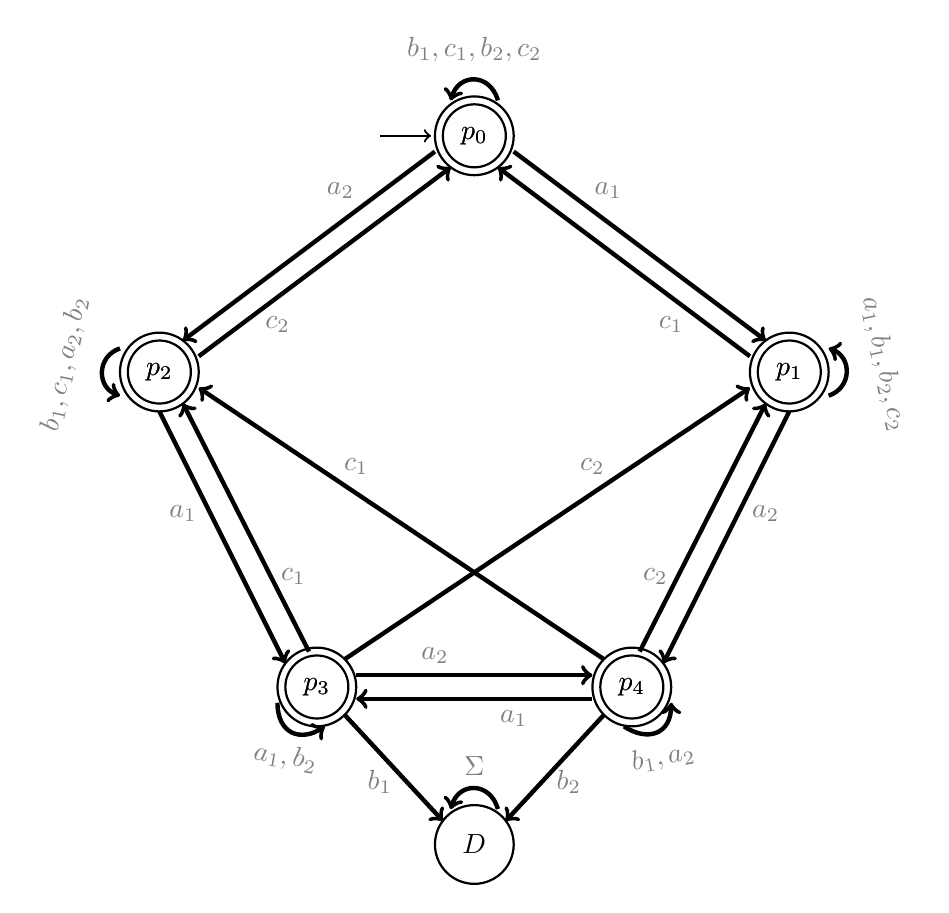
\begin{tikzpicture}
            
            %States
            \draw[thick, ->] (-1.2, 3) -- (-0.55, 3);
            \draw[thick] (0,3) circle (0.5) node {$p_0$};
            \draw[thick] (0,3) circle (0.4) node {$p_0$};
            \draw[thick] (4, 0) circle (0.5) node {$p_1$};
            \draw[thick] (4, 0) circle (0.4) node {$p_1$};
            \draw[thick] (-4, 0) circle (0.5) node {$p_2$};
            \draw[thick] (-4, 0) circle (0.4) node {$p_2$};
            \draw[thick] (-2, -4) circle (0.5) node {$p_3$};
            \draw[thick] (-2, -4) circle (0.4) node {$p_3$};
            \draw[thick] (2, -4) circle (0.5) node {$p_4$};
            \draw[thick] (2, -4) circle (0.4) node {$p_4$};
            \draw[thick] (0, -6) circle (0.5) node {$D$};
            
            %Edges
                %Normal between states
            \draw[ultra thick, ->] (0.5, 2.8) -- (3.7, 0.4);
            \draw[ultra thick, <-] (0.3, 2.6) -- (3.5, 0.2);
            
            \draw[ultra thick, ->] (-0.5, 2.8) -- (-3.7, 0.4);
            \draw[ultra thick, <-] (-0.3, 2.6) -- (-3.5, 0.2);
            
            \draw[ultra thick, ->] (4, -0.5) -- (2.4, -3.7);
            \draw[ultra thick, <-] (3.7, -0.4) -- (2.1, -3.55);
            
            \draw[ultra thick, ->] (-4, -0.5) -- (-2.4, -3.7);
            \draw[ultra thick, <-] (-3.7, -0.4) -- (-2.1, -3.55);
            
            \draw[ultra thick, ->] (-1.5, -3.85) -- (1.5, -3.85);
            \draw[ultra thick, <-] (-1.5, -4.15) -- (1.5, -4.15);
            
            \draw[ultra thick, ->] (-1.65, -4.35) -- (-0.4, -5.7);
            \draw[ultra thick, ->] (1.65, -4.35) -- (0.4, -5.7);
            
                %Diagonal across figure
            \draw[ultra thick, ->] (-1.65, -3.65) -- (3.5, -0.2);
            \draw[ultra thick, ->] (1.65, -3.65) -- (-3.5, -0.2);
            
                %%From state to same state
            \draw[ultra thick, ->] (0.3, 3.45) .. controls (0.2, 3.8) and (-0.2, 3.8) .. (-0.3, 3.45);
            \draw[ultra thick, ->] (4.5, -0.3) .. controls (4.8, -0.2) and (4.8, 0.2) .. (4.5, 0.3);
            \draw[ultra thick, <-] (-4.5, -0.3) .. controls (-4.8, -0.2) and (-4.8, 0.2) .. (-4.5, 0.3);
            \draw[ultra thick, ->] (1.9, -4.5) .. controls (2.2, -4.7) and (2.5, -4.6) .. (2.5, -4.2);
            \draw[ultra thick, <-] (-1.9, -4.5) .. controls (-2.2, -4.7) and (-2.5, -4.6) .. (-2.5, -4.2);
            \draw[ultra thick, ->] (0.3, -5.55) .. controls (0.2, -5.2) and (-0.2, -5.2) .. (-0.3, -5.55);
            
            %Labels
                %From state to other state
            \draw[gray] (1.7, 2.3) node{$a_1$};
            \draw[gray] (-1.7, 2.3) node{$a_2$};
            
            \draw[gray] (2.5, 0.6) node{$c_1$};
            \draw[gray] (-2.5, 0.6) node{$c_2$};
            
            \draw[gray] (3.7, -1.8) node{$a_2$};
            \draw[gray] (-3.7, -1.8) node{$a_1$};
            
            \draw[gray] (2.3, -2.6) node{$c_2$};
            \draw[gray] (-2.3, -2.6) node{$c_1$};
            
            \draw[gray] (0.5, -4.4) node {$a_1$};
            \draw[gray] (-0.5, -3.6) node {$a_2$};
            
            \draw[gray] (1.5, -1.2) node{$c_2$};
            \draw[gray] (-1.5, -1.2) node{$c_1$};
            
            \draw[gray] (1.2, -5.2) node{$b_2$};
            \draw[gray] (-1.2, -5.2) node{$b_1$};
            
                %From state to same state
            
            \draw[gray] (0, 4.1) node {$b_1, c_1, b_2, c_2$};
            \draw[gray] (5.2, 0.1) node[rotate = -78] {$a_1, b_1, b_2, c_2$};
            \draw[gray] (-5.2, 0.1) node[rotate = 78] {$b_1, c_1, a_2, b_2$};
            \draw[gray] (2.4, -4.9) node[rotate = 10] {$b_1, a_2$};
            \draw[gray] (-2.4, -4.9) node[rotate = -10] {$a_1, b_2$};
            \draw[gray] (0, -5) node {$\Sigma$};
            
            
        \end{tikzpicture}
    \end{center}
    \caption{Final state machine for $\mathbf{M}$. Combined with table \ref{tab:Mstates} the following state pattern can be noted. Top: Both variables are equal with a value of zero. Top middle: One of the variables is nonzero, the other is zero. Bottom middle: Both variables are non zero, but different values.  Bottom: Dead state (a test did not match current properties).}
    \label{fig:M}
\end{figure}
